\begin{thm}{043}{\hosi 8\maru}{東大}
 座標平面において、媒介変数$t~(0\le t< 2\pi)$を用いて、$x=\cos2t$, $y=t\sin t$と表される曲線が囲む領域の面積を求めよ。
\end{thm}

まず、$x, y$の増減を考える。
\[ \frac{dx}{dt}=-2\sin 2t, \quad  \frac{dy}{dt}=\sin t+t\cos t \]
$\dfrac{dy}{dt}=0$となるときの$t$の値について考える。明らかに$t\neq \dfrac{\pi}{2}, \dfrac{3\pi}{2}$なので、求める$t$は$t=-\tan t$の解である。$y=x$と$y=-\tan x$のグラフの交点を考えることにより、$\dfrac{\pi}{2}$から$\pi$の間と$\dfrac{3\pi}{2}$から$2\pi$の間にそれぞれ1つずつ解が存在することがわかる。これらをそれぞれ$\alpha$, $\beta$とおく。これを用いて増減は以下のようにまとめられる。
\begin{align*}
\begin{array}{c|c|c|c|c|c|c|c}
 t & 0 & \cdots & \dfrac{\pi}{2} & \cdots & \alpha & \cdots & \pi \\[1.0ex] \hline
 \dfrac{dx}{dt} & 0 & - & 0 & + & + & + & 0 \\[1.0ex] \hline
 \dfrac{dy}{dt} & 0 & + & + & + & 0 & - & - \\[1.0ex] \hline
 (x, y) & \cdot & \nwarrow & \uparrow & \nearrow & \to & \searrow & \downarrow \\ \hline\hline
 t & \pi & \cdots & \dfrac{3}{2}\pi & \cdots & \beta & \cdots & 2\pi \\[1.0ex] \hline
 \dfrac{dx}{dt} & 0 & - & 0 & + & + & + & 0 \\[1.0ex] \hline
 \dfrac{dy}{dt} & - & - & - & - & 0 & + & + \\[1.0ex] \hline
 (x, y) & \downarrow & \swarrow & \downarrow & \searrow & \to & \nearrow & \uparrow \\
 \end{array}
\end{align*}
これを踏まえてグラフの概形を書く。点A$(1, 0)$ $[t=0]$からはじめ、点B$\left(-1, \dfrac{\pi}{2}\right)$ $\left(t=\dfrac{\pi}{2}\right)$、点C$(\cos2\alpha, \alpha\sin\alpha)$ $(t=\alpha)$、点A$(1, 0)$ $(t=\pi)$、点D$\left(-1, -\dfrac{3\pi}{2}\right)$ $\left(t=\dfrac{3\pi}{2}\right)$、点E$(\cos2\beta, \beta\sin\beta)$ $(t=\beta)$、点A$(1, 0)$ $(t=2\pi)$を順に通る。加えて$0\le t \le \dfrac{\pi}{2}$のとき、
\begin{align*}
 (\pi-t)\sin{\pi-t}-t\sin t=(\pi-2t)\sin t \ge 0
\end{align*}
であるから経路BCAは経路ABよりも常に上にあり端点以外で交わらない。また、$\pi\le t\le \dfrac{3}{2}\pi$のときは、$t=\pi+\alpha$とおけば$0\le\alpha\le\dfrac{\pi}{2}$で、
\begin{align*}
 (2\pi-\alpha)\sin(2\pi-\alpha)-&(\pi+\alpha)\sin(\pi+\alpha) \\
 &=-(\pi-2\alpha)\sin\alpha \ge 0
\end{align*}
であるから経路ADは経路DEAよりも常に上にあり端点以外で交わらない。

\begin{wrapfigure}[10]{r}[0pt]{80pt}
 \centering
 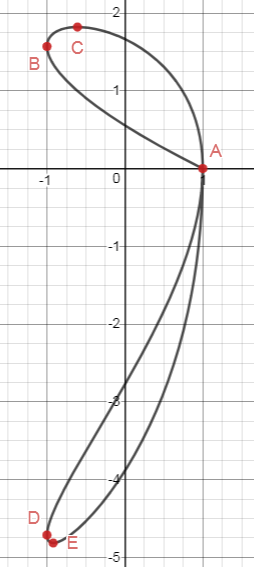
\includegraphics[width=\linewidth]{../problems/Q_043/A_043.png}
\end{wrapfigure}
このことから、グラフは右図のようになることがわかる。これによって囲まれる面積を求めるには、$y\ge 0$と$y\le 0$の二つの領域に分けて考えて、
\begin{align*}
 (y\ge 0): \quad & \int_{\mr{B}\to \mr{C}\to \mr{A}}\!\!\! y \,dx - \int_{\mr{B}\to \mr{A}}\! y \,dx \\
 (y\le 0): \quad & \int_{\mr{D}\to \mr{A}}\! y \,dx - \int_{\mr{D}\to \mr{E}\to \mr{A}}\!\!\! y \,dx
\end{align*}
とすればよい。このとき、
\begin{align*}
 &\int\! y \,dx = \int\! y(t) \frac{dx}{dt} \, dt \\
 =& \int\! t\sin t \cdot (-2\sin2t) \,dt \\
 =& \int\! (-4t\sin^2t\cos t) \,dt \\
 =& \left[-\frac{4}{3}t\sin^3t\right] - \int\! \left(-\frac{4}{3}\sin^3 t\right) \,dt \\
 =& \left[-\frac{4}{3}t\sin^3t\right] - \left[\frac{4}{3}\cos t -\frac{4}{9} \cos^3t\right]
\end{align*}
と計算される。以上のことを用いて求める面積は、
\begin{align*}
 \left(\int_{\frac{\pi}{2}}^\pi\! y \,dx - \int_{\frac{\pi}{2}}^0\! y \,dx \right) + \left(\int_{\frac{3}{2}\pi}^\pi\! y \,dx - \int_{\frac{3}{2}\pi}^{2\pi}\! y \,dx \right) = \frac{32}{9}
\end{align*}
